\documentclass[12pt]{article}

\usepackage[utf8]{inputenc}
\usepackage[T1]{fontenc}
\usepackage{geometry}
\usepackage{graphicx} %figures
\usepackage{subfig} %subfigures
\usepackage{gensymb} %degree sign
\usepackage{amsmath} %math stuff
\usepackage{bm} %bold stuff
\usepackage[]{algorithm2e} %algorithms
\geometry{a4paper}

\title{Part 16: Monte Carlo Based Bayesian Acquisition Functions}

\begin{document}
\date{March 22, 2021}
\maketitle

Hey everyone sorry for the one week delay in posting. I wasn't happy with the results from last week and wanted another week to work on this stuff. As an apology I have another post coming out today (Post 17) about linear basis functions that's a light read and a lot of ``fun''. Today we will be tackling the difficult subject of acquisition functions for Bayesian optimization that can only be solved with monte carlo methods.

\section{q-EI}

The first acquisition function we'll talk about is multi-expected improvement (q-EI) where the $EI(x)$ function is solved for q sets of inputs $x$:

\begin{equation}
EI(x)=E_y[max\{(y-max(Y))^+\}]
\end{equation}

\vspace{5mm}

Where we want to maximize $EI(x)$ to improve a function $y=f(x)$. Of course the ``improvement'' is $y-max(Y)$ but the ``expected'' is $E_y[...]$ because we have a probabilistic model (in this case a GP or Gaussian process model) which has been talked about at length previously. For a single and double recommendation $q=1,2$ this has an analytical form:

\begin{align*}
EI(x,q=1)=(y(x)-max(Y))\Phi(z(x))+\sigma(x) \phi(z(x))
\end{align*}
\begin{align*}
z(x)=\dfrac{y(x)-max(Y)}{\sigma(x)}
\end{align*}
\begin{align*}
EI(x,q=2)=(y(x_1)-max(Y))*I_1+(y(x_2)-max(Y))*I_2
\end{align*}

\vspace{5mm}

Where $I_i$ indicate whether a point $x_i$ is better than both $max(Y)$ and the other points $x_j$ (Ginsbourger 2008). For the example problem in Figure 1 I have plotted EI in Figure 2a. 

\begin{figure}[h]
\centering
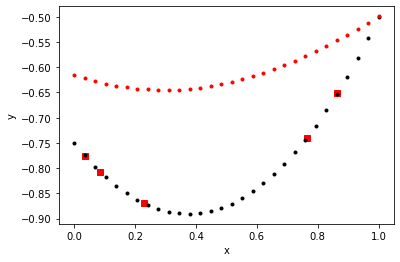
\includegraphics[width=0.6\textwidth]{Post_16_funct}
\caption{Toy Problem | Black is $f(x)$, Red is GP approximation of $f(x)$}
\end{figure}

Luckily for us this can be reasonably generalized to any $q-EI(x)$ by solving Equation (1) using an $M$ monte carlo sample (random sample) of the posterior of the GP:

\begin{align*}
q-EI(x)=M^{-1} \Sigma_{i=1}^M(max\{y(x)-max(Y)\})^+_i
\end{align*}

\vspace{5mm}

Think about $q-EI(x)$ like an algorithm first. For $M$ samples of the posterior of the GP (GPs are statistical models after all so they should have distributions) we can sample a resultant $y$ given some vector of $x$. We then take the maximum of this improvement vector and pass it through our RELU operator (if the input is less than 0 the output is set to 0, otherwise nothing occurs). We do this $M$ times given a monte carlo average of the EI for a given $x$. 

\vspace{5mm}

How do we sample $y$? We will use what is termed the reparameterization trick for some posterior covariance $C$: $y \sim GP(\mu,C) \rightarrow \mu + Lz$ where $LL^T=C$ (Cholesky Decomposition). The matrix $C$ is defined as follows:

\begin{align*}
C(x,x')=K(x,x)-K(x,x')(K(x',x')+\sigma^2 I)^{-1}K(x,x')^T
\end{align*}

\vspace{5mm}

For any covariance kernel $K(x,x')$ which we have gone over. In this case $x$ is the input data we want to get the covariance of and $x'$ is the data we already have. So in that algorithm I mentioned above, when we generate our $M$ samples, we do so using this matrix $C$ and a multivariant normal vector $z$. Note that in order to solve $LL^T=C$ in the code I had to add a small amount of jitter $L=Chol(C+10^{-4}I)$.

\section{q-KG}

The next acquisition function is based on the ``knowledge gradient'' problem:

\begin{equation}
KG(x)=E_y[max_{y'}\{(y' | y)^+\}]
\end{equation}

\vspace{5mm}

The idea here is we want to maximize $KG(x)$ which is the expectation (average) over our current data set $Y$ of the maximum of a ``fantasy'' data set $Y'$. In English, this means we want to maximize the ``next-step'' potential of our current data set by projecting forward for additional maximization. So by pretending our current data set is made up of some fantasy points, we condition on those points and maximize the average of the result:

\begin{align*}
q-KG(x)=F^{-1} \Sigma_{f=1}^F [M^{-1}\Sigma_{j=1}^M max\{y_j\}] | x_f
\end{align*}

\vspace{5mm}

The reason this one is harder to compute than the EI ones is that KG requires two ``steps'', which itself requires conditioning on fake data. Also note that we use the reparameterization trick as before for some posterior covariance $C$: $y \sim GP(\mu,C) \rightarrow \mu + Lz$ where $LL^T=C$. Also note that for the fake fantasy data I use the mean prediction in the GP and recalculate $C$ as $x'=\{x',x_f\}$.

\vspace{5mm}

The results are in Figure 2c for the toy problem described in Figure 1. There are two massive things I left out of this discussion: (i) hyperparameter optimization and (ii) acquisition function optimization. So the model itself sucks (part (i)) and we don't have a true ``optimum'' (part (ii)). This is okay because over the next few week we will be focusing on the details of solving difficult multi-fidelity optimization problems. This will go as follows':

\begin{itemize}
  \item The Multi-Fidelity Kernel and Likelihood
  \item Hyperparameter Optimization
  \item The Multi-Fidelity Gradient and $\mu$ Optimization
  \item q-KG Acquisition Function using MC + Gradient
  \item q-KG Optimization
\end{itemize}

\begin{figure}[h]
\centering
\subfloat[][Analytical EI]{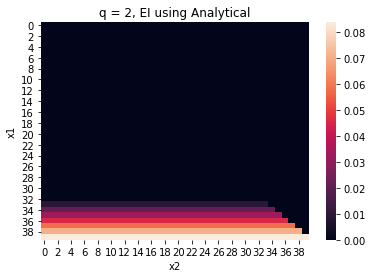
\includegraphics[width=0.3\textwidth]{Post_16_EI1}}
\subfloat[][MC 2-EI]{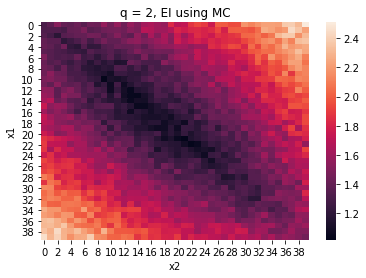
\includegraphics[width=0.3\textwidth]{Post_16_EI2}}
\subfloat[][MC 2-KG]{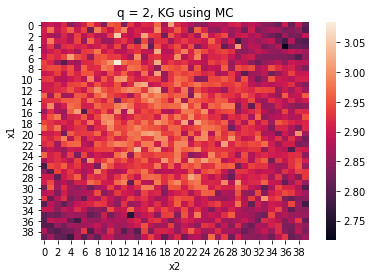
\includegraphics[width=0.3\textwidth]{Post_16_EI3}}
\caption{Acquisition Functions}
\end{figure}

\end{document}